\section{Einleitung}

\begin{frame}{Einleitung}
    \textbf{Ziel:} Erkennen von Nummernschildern auf Fotos und Auslesen der Nummernschilder
    
    Arafat et al. (2019):\\
\textit{Systematic review on vehicular licence plate recognition framework in intelligent transport systems}~\cite{arafat}
    
    \textbf{Herausforderungen:}
    \begin{itemize}
        \item Vielfältigkeit der Nummernschilder
        \item Rahmenbedingungen der Bildaufnahme (Beleuchtung)
    \end{itemize}
\end{frame}

\begin{frame}{Beispiel}
  \begin{figure}
    \begin{center}
      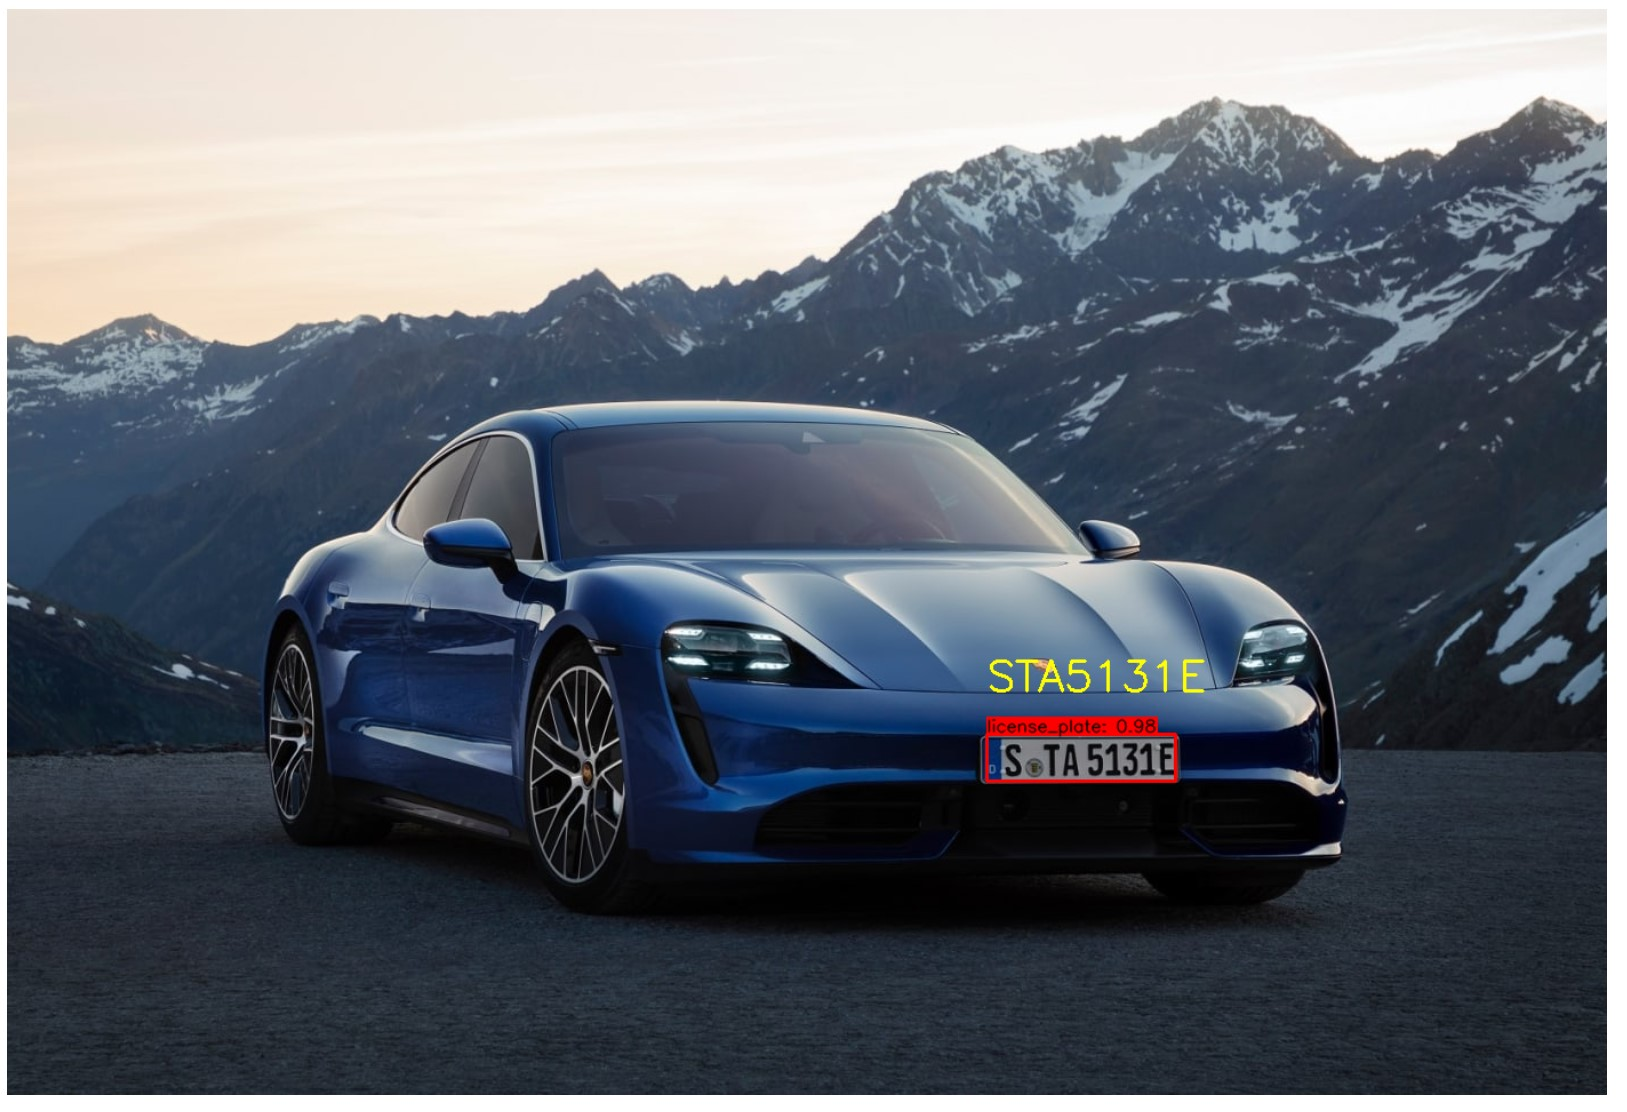
\includegraphics[width=0.8\textwidth]{bilder/Bild2}
      \caption{Beschreibung
      \footnote{Bildquelle: \url{https://github.com/theAIGuysCode/yolov4-custom-functions}}}
    \end{center}
  \end{figure}
\end{frame}

\begin{frame}{Yolo}
    
    Auffassung der Objekterkennung als Regressionsproblem 
    
    Charakteristika:
    \begin{itemize}
        \item System zur Objekterkennung 
        \item Generierung potenzieller Bounding Boxes in einem Bild
        \item Klassifizierung
    \end{itemize}
\end{frame}